\documentclass{article}

% if you need to pass options to natbib, use, e.g.:
%     \PassOptionsToPackage{numbers, compress}{natbib}
% before loading neurips_2021

% ready for submission
\usepackage{neurips_2021}

% to compile a preprint version, e.g., for submission to arXiv, add add the
% [preprint] option:
%     \usepackage[preprint]{neurips_2021}

% to compile a camera-ready version, add the [final] option, e.g.:
%     \usepackage[final]{neurips_2021}

% to avoid loading the natbib package, add option nonatbib:
%    \usepackage[nonatbib]{neurips_2021}

\usepackage[utf8]{inputenc} % allow utf-8 input
\usepackage[T1]{fontenc}    % use 8-bit T1 fonts
\usepackage{hyperref}       % hyperlinks
\usepackage{url}            % simple URL typesetting
\usepackage{booktabs}       % professional-quality tables
\usepackage{amsfonts}       % blackboard math symbols
\usepackage{nicefrac}       % compact symbols for 1/2, etc.
\usepackage{microtype}      % microtypography
\usepackage{xcolor}         % colors
\usepackage{cite}
\usepackage{biblatex} %Imports biblatex package
\addbibresource{ref.bib} %Import the bibliography file
\usepackage{graphicx}
\usepackage{authblk}
\title{Assessment of Heart Rate and Risk Analysis of Cardiac Disorders using Supervised Learning :\\ \href{https://github.com/Sanatan-Shrivastava/CST403-PR}{github link}}


% The \author macro works with any number of authors. Ther}e are two commands
% used to separate the names and addresses of multiple authors: \And and \AND.
%
% Using \And between authors leaves it to LaTeX to determine where to break the
% lines. Using \AND forces a line break at that point. So, if LaTeX puts 3 of 4
% authors names on the first line, and the last on the second line, try using
% \AND instead of \And before the third author name.


% \author{
%   Rahul Singh Tanwar\\
%   Department of Computer Science\\
%   Cranberry-Lemon University\\
%   Pittsburgh, PA 15213 \\
%   \texttt{hippo@cs.cranberry-lemon.edu} \\
%   examples of more authors
%   \And
%   Coauthor \\
%   Affiliation \\
%   Address \\
%   \texttt{email} \\
%   \AND
%   Coauthor \\
%   Affiliation \\
%   Address \\
%   \texttt{email} \\
%   \And
%   Coauthor \\
%   Affiliation \\
%   Address \\
%   \texttt{email} \\
%   \And
%   Coauthor \\
%   Affiliation \\
%   Address \\
%   \texttt{email} \\
% }




\begin{document}

\maketitle

\begin{abstract}
  This paper deals with assessment of heart rate and risk analysis of cardiac disorders with the help of machine learning. Some of the supervised machine learning techniques used in this prediction of heart disease are random forest (RF), support vector machine (SVM), naive Bayes (NB) and k-nearest neighbour (KNN) algorithm. Maximum accuracy of 95.08\% was achieved by using the Random Forest algorithm.
\end{abstract}

\section{Introduction}
Predicting and detection of heart disease has always been a critical and challenging task for healthcare practitioners. Hospitals and other clinics are offering expensive therapies and operations to treat heart diseases. So, predicting heart disease at the early stages will be useful to the people around the world so that they can take necessary actions before getting severe. Heart disease is a significant problem in recent times; the main reason for this disease is the intake of alcohol, tobacco, and lack of physical exercise. Over the years, machine learning shows effective results in making decisions and predictions from the broad set of data produced by the healthcare industry. This paper includes the literature survey done in this project and also the machine learning algorithms used to train the model.

\section{Related Work}

 \cite{rt1} Aims to develop a model that predicts the prevalence of cardiovascular disease using health-related data that can be easily measured by smartwatch users. To classify the prevalence of cardiovascular disease with health related variables extracted from smartwatch, machine learning classification techniques like logistic regression, artificial neural network and support vector machine were used. Out of the three classification techniques, the support vector machine classification provided the best accuracy. In this paper, nine input variables were selected from the Korea National Health and Nutrition Examination Survey 2019 data in consideration of functions that can be measured in Samsung Electronics’ smartwatches.

Cardiac arrhythmia is defined as a set of conditions related to irregular heart-rate. In \cite{rt2} the author highlighted the risk of Cardiac arrhythmia, It is the most prevalent cause of natural death worldwide. In \cite{rt2} the research aims to develop a model for classification of Cardiac arrhythmia. The model developed using Random Forest Classifier model on features having the most impact on CA such as respiratory rate, blood pressure, sodium, potassium, calcium, among the other features. Widely used open MIMIC-III database is used which consists of a large number of clinical monitor data of ICU Patients. The following model has  left behind a previously built model with 98\% accuracy.

In \cite{rt6}, authors have discussed a model which demonstrates heart rate as a risk factor for cardiac disorders. The authors have worked on meta-regression of randomised health variables which predicts the risk of cardiac disorders due to heart rate. Various studies concluded that increase in heart rate is an independent risk factor for various cardiovascular diseases along with various others like increase in blood pressure, cholesterol, cardiac dysfunction and diabetes. Heart rate is an important risk factor in the patients having coronary artery diseases. Heart rate is also a predictor of short-time coronary events like cardiovascular syndromes, myocardial infarction and sudden cardiac death. The heart rate reduction is obtained without any effect on the sympathetic activity or contractility.

Author \cite{rt3} in this article have discussed epidemiological studies that aimed to find the relationship between heart rate and all-cause or cardiovascular disorder and mortality, reporting that a high heart rate was linked with a higher risk of mortality and cardiovascular cases. This relationship has been found to be generally stronger in men than among women. The increase in the cardiovascular risk is directly linked with the increasing heart rate, and also increase in high blood pressure. In this article the author analyzes that an increase in heart rate by 10 beats per minute was associated with an increase in the risk of cardiac death by at least 20\%, and increased risk has been observed with an increase in systolic blood pressure by 10 mm Hg. It has also been shown that heart rate recorded in elderly men has a strong predictive value in survival to a very old age. Taken together, these results indicate that the risk associated with accelerated heart rate is not only statistically significant but also clinically relevant and that it should be taken into account in the evaluation of the patients. Although the association between elevated heart rate and cardiovascular morbidity and mortality has been demonstrated in a large number of epidemiological studies, tachycardia has remained a neglected cardiovascular risk factor until very recently. For the first time, the recent guidelines of the European Society of Cardiology and the European Society of Hypertension indicate that an accelerated heart rate is considered as an independent risk factor and potentially as a target for pharmacologic therapies, especially in high-risk patients.

Both medical and affective computing applications can benefit greatly from remotely assessing physiological activity. Different approaches for the unobtrusive detection of heart rate (HR) utilising human facial recordings have been proposed in a study recently. These techniques rely on minor colour changes or facial gestures caused by cardiovascular activity, which are imperceptible to the naked eye but may be caught by digital cameras. Signal processing and machine learning are two ways that have been presented \cite{rt4}. However, because these strategies are tested on diverse datasets, there is no consensus on how well they function. Face video processing, face blood volume pulse (BVP) signal extraction, and HR computation are the three phases of the general HR processing pipeline. According to each level, the approaches provided in the study are classified and grouped. Using the public database MAHNOB-HCI, algorithms are analysed and compared at each level based on their performance. This article's findings are limited to the MAHNOB-HCI dataset. The removed facial skin area has greater BVP information, according to the results. 

For estimating HR, blind source separation and peak detection approaches are more robust with head motions \cite{rt4}.
The heart rate (HR) is a measure of physiological activity that can reveal information about a person's health and mood (Malik, 1996; Armony and Vuilleumier, 2013). Physical activity, emotional stress, and medications all have an impact on heart functions. As a result, HR data can be used for a variety of purposes, including medical diagnosis, fitness assessment, and emotion recognition. Electronic or optical sensors are used in traditional HR measurement methods. Electrocardiograms (ECGs), sphygmomanometry, and pulse oximetry, the latter of which produces a photoplethysmogram, all require skin contact (PPG) \cite{rt5}.

In \cite{rt7} the authors have used an R studio rattle to perform heart disease classification of the UCI dataset. It provides a visual representation of the dataset, working environment and building the predictive analytics. The process of machine learning initiates from a pre-processing data phase followed by feature selection based on DT entropy, classification of modeling performance evaluation, and the results with better accuracy. In \cite{rt8} authors have developed a random forest model implemented in a Python programming package.A grid search algorithm is used for tuning the model hyperparameters. The best heart failure detection accuracy of 90\% is obtained using tuned hyperparameters.


\section{Problem}

\subsection{Problem Statement}
Assessment of Heart Rate and Risk Analysis of Cardiac Disorders using Supervised Learning.

\subsection{Problem defination}
This project aims to detect and predict various cardiac disorders using Supervised Learning. More precisely, this system takes in various physiological parameters’ data and then based on the trained model, predicts whether that particular person has heart disease or not.

\section{Problem Formulation}
To predict whether any person has cardiac disorder or not, this algorithm is initially trained on a dataset which has 13 different types of input features (physiological parameters). After training, new data is given to the trained model and the model predicts whether a person has heart disorder or not. The idea that makes this project unique is the collection of a wide variety of algorithms. As opposed to other solutions proposed in earlier literature, this project uses a wide variety of algorithms for training. A total of four different algorithms are used. Based on these algorithms, four different models were created. Finally, the accuracies provided by these four different models were compared.

\section{Methodology}

\subsection{K-Nearest Neighbour}

K-Nearest Neighbour is Machine Learning algorithms based on Supervised Learning technique.
The K-NN algorithm assumes the similarity between the new case/data and available cases and puts the new case into the category that is most similar to the available categories.
K-NN algorithm stores all the available data and classifies a new data point based on the similarity. This means when new data appears then it can be easily classified into a well suited category by using K- NN algorithm.The K-NN algorithm can be used for Regression as well as for Classification. K-NN is a non-parametric algorithm, which means it does not make any assumption on underlying data. It is also called a lazy learner algorithm because it does not learn from the training set immediately instead it stores the dataset and at the time of classification, it performs an action on the dataset. The KNN algorithm at the training phase just stores the dataset and when it gets new data, then it classifies that data into a category that is much similar to the new data.Accuracy achieved by K-Nearest Neighbor (KNN) Algorithm is 67.21\%.

\textbf{Working}
\begin{enumerate}
    \item Select the number K of the neighbors
    \item Calculate the Euclidean distance of K number of neighbors
    \item Take the K nearest neighbors as per the calculated Euclidean distance.
    \item Among these k neighbors, count the number of the data points in each category.
    \item Assign the new data points to that category for which the number of the neighbor is maximum.
    \item Our model is ready.
\end{enumerate}


\subsection{Naive Bayes Classifier }
Naive Bayes is a method to predict the probability of output based on various attributes. This algorithm is mostly used in classification and with problems having multiple classes.In this algorithm we use a probabilistic approach for classification.It is easy and fast to predict the class of the test data set. It also performs well in multi-class prediction. When assumption of independence holds, a Naive Bayes classifier performs better compared to other models like logistic regression and less training data is needed.Accuracy achieved by Naive Bayes Algorithm is 85.25%.

\textbf{Working}\\
In the naive bayes algorithm we are given a set of input features and one output feature.Suppose we are given n input features say x1,x2,x3,.......xn and one output feature y and we have to find the value of P(y | x1 x2 x3 …… xn) which we can find with the help of equation 1. This formula is called bayes theorem and we are using the principle of conditional probability. 

\begin{figure}[h]
    \centering
    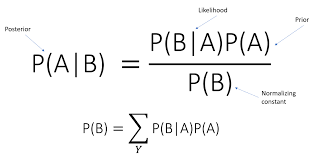
\includegraphics[scale=0.88]{nb.png}
    \caption{Naive Bayes}
\end{figure}


\subsection{Support Vector Machine (SVM)}

Support Vector Machine is one of the most popular algorithms of machine learning. It is used for classification as well as regression problems. SVM creates a decision boundary that can segregate n-dimensional space into classes. This decision boundary is called a hyperplane. This hyperplane is chosen in a way to maximise the margin. The data points which are on the edges of the margin from the hyperplane are known as support vectors. There are mainly two types of SVM, that are popularly known as Linear and Non Linear SVM. Linear, Poly, RBF and Sigmoid are the kernels that are used with SVM.


\begin{figure}[h]
    \centering
    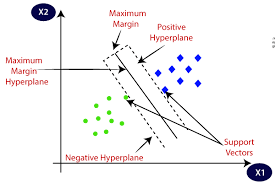
\includegraphics[scale=0.88]{svm.png}
    \caption{Support Vector Machine}
\end{figure}


For this project, Linear and RBF kernels were used to train the model. The accuracy achieved by Linear SVM on test data was 86.69\% and that on the RBF kernel was 90.16\% as shown in figure below

\begin{figure}[h]
    \centering
    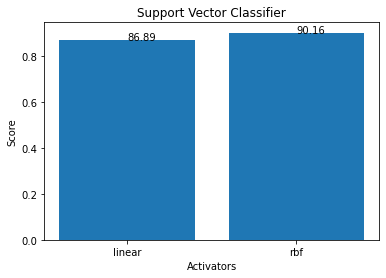
\includegraphics[scale=0.50]{svmscu.png}
    \caption{Accuracy using SVM}
\end{figure}


\subsection{Random Forest}
Random Forest is a supervised machine learning algorithm that is widely used for classification problems Random Forest is developed by the help of Decision Trees. For training, bagging method is used. Hence Random Forest builds multiple decision trees and then merges them to get a better prediction. It also works well on huge databases. As the forest grows, it generates an internal unbiased estimate of the generalisation error. Also, It offers a method for guessing missing data that works well and retains accuracy even when a high percentage of the data is missing.

\begin{figure}[h]
    \centering
    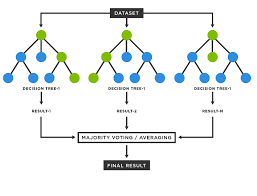
\includegraphics[scale=1]{renfor.png}
    \caption{Random Forest}
\end{figure}

The forests that are created can be preserved and used on other data in the future. Random Forest also includes techniques for balancing error in uneven data sets with a class population. After training data using the Random Forest, the accuracy achieved on test data was 95.08\%.

\section{Experiments}\\
\cite{linkdata} dataset was used to train the models. This dataset contains a total of 303 samples. Each sample consists of 13 input features and one output variable. The input features are age, sex, chest pain, resting blood pressure, serum cholesterol levels, fasting blood sugar levels, resting electrocardiographic results, maximum heart rate achieved, exercise induced angina, oldpeak, slope of the peak exercise ST segment, number of major vessels and thal.

\begin{figure}[h]
    \centering
    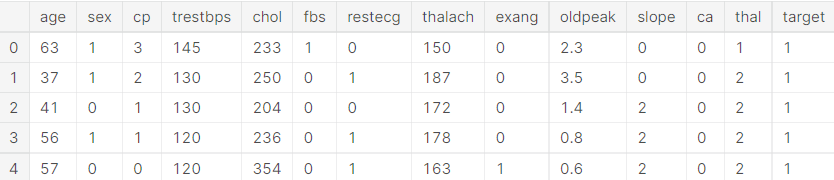
\includegraphics[scale=0.70]{table.png}
    \caption{Data set}
    \label{fig:dataset}
\end{figure}

To better understand the correlation between input features and target, some plots were plotted.Fig. 7 shows the relationship between ages and heart disease. Also, Fig. 6 shows the relationship between gender and disease. 

\begin{figure}[h]
    \centering
    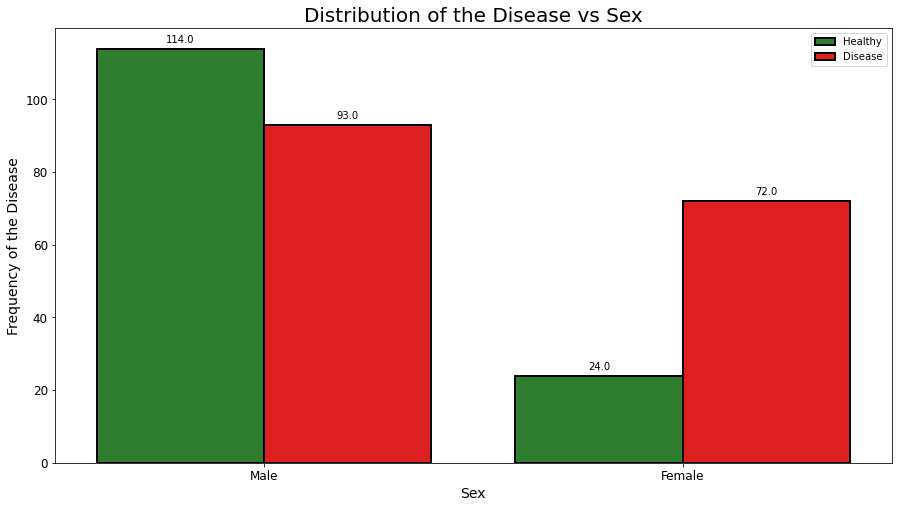
\includegraphics[scale=0.30]{__results___11_1.png}
    \caption{Distribution}
    \label{fig:dis}
\end{figure}

\begin{figure}[h]
    \centering
    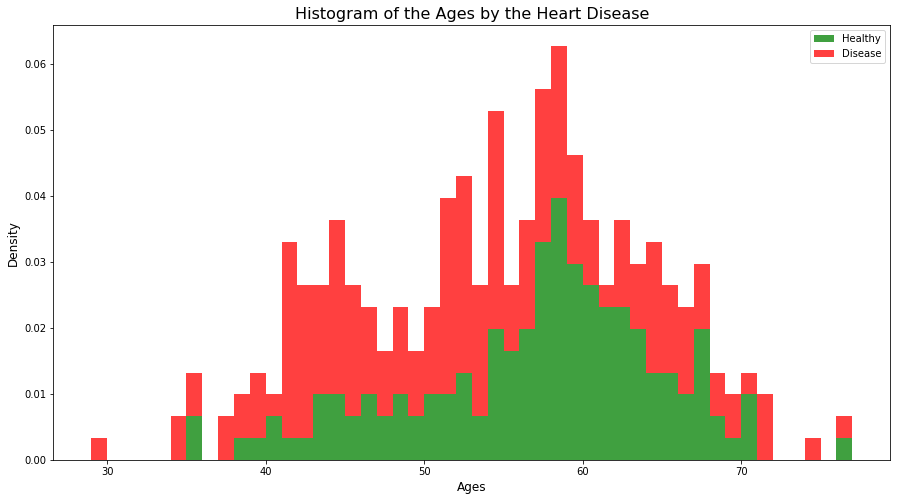
\includegraphics[scale=0.30]{__results___9_0.png}
    \caption{Distribution}
\end{figure}


\section{Results and Discussion}

After training the model on training data, it was tested on testing data and the accuracy given by all the 4 models is shown in below fig.
\begin{figure}[h]
    \centering
    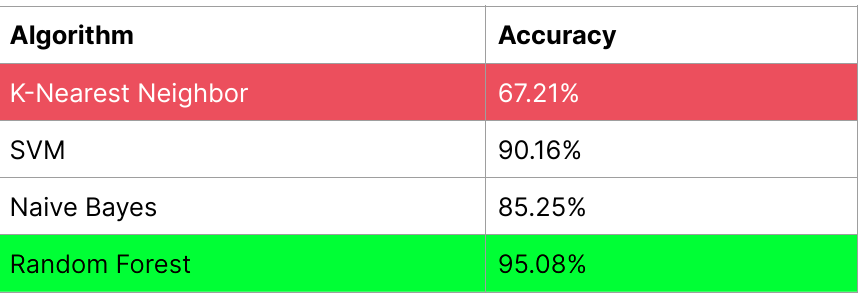
\includegraphics[scale=0.30]{Screenshot from 2021-12-12 10-45-18.png}
    \caption{Distribution}
\end{figure}

As depicted in the figure, K-Nearest Neighbor has the lowest accuracy of 67.21\%. On the other hand, the highest accuracy of 95.08\% is achieved by using Random Forest. SVM and Naive Bayes algorithms also showed a decent performance with accuracies of 90.16\% and 85.25\% respectively. So, random forest seems to be a clear winner for this project in terms of accuracy. Apart from the accuracy, because Random Forest is also known for performing well on huge datasets, it would be an added advantage.
The aim of this project was to predict the heart disease of any particular person. After training the model with Random Forest, the model is predicting the results with over 95\% accuracy. This seems to be a good model and a good companion to anyone who wants to predict heart disease.

\section{Conclusion}

Conclusion : 
In conclusion of this report we can say that the Random Forest model gives the highest accuracy and is the best model for predicting heart disorders and it can be used for a large dataset. The health industry normally demands for a higher accuracy and hence even if it is giving accuracy of 95.08\% but still there is a scope for improvement. This accuracy can be improved by fine tuning the hyper parameters. Also, it might be possible that accuracy may be further increased by creating any hybrid model. 


\printbibliography 
\end{document}